\section{Estudio de Mercado}

\subsection{Definición del Producto}

Debido al gran aumento en  bandas emergentes que se ha notado en la V región,
surge la idea de poder integrar servicios existentes de apoyo a dichas bandas,
más nuevas ideas para ayudar al crecimiento de las bandas de la región.

\emph{Music Labs} será un servicio que reúna los elementos básicos para poder lanzar
a la fama a una banda emergente como:
\begin{itemize}
	\item Sala de ensayo
	\item Estudio de grabación
	\item Salón de eventos
	\item Asesoría personal
	\item Posicionamiento Web 2.0
\end{itemize}

Tanto el estudio de grabación como la sala de ensayo ofrecerán soporte y asesoría
técnica completa a cada banda, para poder obtener un trabajo de alta calidad.


El salón de eventos va a servir para ser la primera instancia de interacción de
las nuevas bandas con su público, ya que luego serán puestos en contacto con
distintos lugares en la zona, que son conocidos por ser la cuna para nuevas bandas.

La asesoría personal es muy similar a lo que podría ser un Mánager,
pero en este caso \emph{Music Labs} irá más allá, transformando esta figura,
en un asesor completo para las nuevas bandas,
ya que cada asesor estará respaldado por un grupo de profesionales, con experiencia en el área.

Finalmente el posicionamiento web 2.0, es una herramienta vital en el día de hoy,
debido a los grandes impactos provocados por las redes sociales.
Se ofrecerá tanto la asesoría para realizar el sitio oficial de la banda en internet,
como el posicionamiento en las distintas redes sociales, como Twitter, Facebook, MySpace, etc.

\emph{Music Labs} contará con expertos en cada área para proveer un servicio de excelencia.
Principalmente el unir estos servicios existentes (por separado),
es para poder evitar el procedimiento de buscar en distintas fuentes,
elementos que sirvan a la banda para alcanzar un solo objetivo.

Los servicios podrán ser contratados individualmente o en grupos,
ya que para \emph{Music Labs} es muy importante poder desligar de cualquier actividad que no tenga
que ver con la composición musical y el realizar música a las nuevas bandas por que muchas
de aquellas actividades quitan el tiempo a la banda, atrasando su despegue a la fama de una
manera notoria.

Los precios se fijaran de acuerdo a los valores de la competencia,
para de esta manera ofrecer la mejor oferta en el mercado.

Por otro lado se harán distintos descuentos dependiendo de la cantidad de servicios que se requiera contratar,
entre otras cosas.

Para facilitar el pago del o los servicios habrán varias modalidades de pago para adecuarse
a cada cliente en particular y se ofrecerán distintos plazos dependiendo de la cuota,
de los servicios requeridos, el numero de integrantes de la banda, los profesionales requeridos, entre otros.

En la actualidad internet es donde más se encuentra información sobre bandas emergentes,
es por esto que se hará una campaña publicitaria que constará de 3 pasos para posicionar
en la V región a \emph{Music Labs} como empresa del mercado musical. Primero se hará publicidad en las redes
sociales  para dar a conocer sin dar mayores detalles de la empresa \emph{Music Labs},
de esta forma se pretende atraer a posibles clientes curiosos por saber más sobre la empresa.

Segundo se publicará en diarios, revistas y/o cualquier medio que atraiga potenciales clientes,
dando a conocer más detalles de los servicios que se ofrecerán y/o descuentos para los primeros clientes.

Y tercero para inaugurar el lugar físico de \emph{Music Labs} se hará una fiesta (\emph{Music Labs Party})
en donde se presentará finalmente la empresa, además se invitará a personajes musicales influyentes
dentro de la V región para promocionar \emph{Music Labs}.

\emph{Music Labs} estará ubicado en el centro de la cuidad de Viña del Mar cercano a la plaza de Viña del Mar,
en donde se encontrara la oficina de asesoramiento, sala de ensayos, estudio de grabación y salón de eventos.

En primera instancia \emph{Music Labs} proveerá sus servicios dentro de la V región específicamente Valparaíso - Viña del Mar
debido a que solo en esta zona se encuentra las dependencias antes mencionada,
posteriormente se podría lanzar Musica Labs en otra región.

Sin embargo si bien \emph{Music Labs} se encuentra en Viña del Mar,
gracias a las redes sociales y el sitio Web se darán a conocer las bandas emergentes a nivel nacional
para que alcancen la fama.


\subsection{Mercado Objetivo}

El mercado musical siempre ha sido un tema de interés dentro de lo que es la población adulto-joven de Chile,
en especial dentro de la región de Valparaíso, debido a la gran afluencia de gente en la vida nocturna,
la cantidad de universidades e institutos de educación superior en la región,
dando como consecuencia un flujo creciente de gente interesada en la música.

Algo que marca lo anteriormente dicho, son los variados eventos durante el año que tienen como objetivo
difundir tanto la musica local, como de todo el país. Evento como el ``Rockodromo'', ``Rock Carnaza'',
organizados por las ``Escuelas del Rock''~\footnote{\url{http://www.escuelasderock.cl/}},
los carnavales culturales, etc, los cuales captan la atención y participación de jóvenes como
adultos.

Basándonos en los estudios del último CENSO realizado el año 2002,
se puede tener una estimación de la relación que existe entre los grupos socioeconómicos
en la V región, donde se puede notar la mayor cantidad de habitantes en la zona, por grupo.

\begin{figure}[h!]
    \centering
	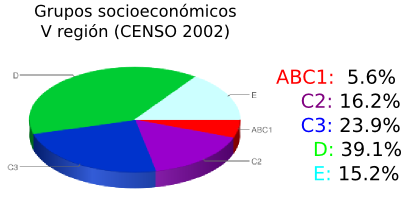
\includegraphics[width=0.6\textwidth]{img/grupos_soc}
  \caption[Porcentaje de grupos socioeconómicos de la V región]{Porcentaje de
  grupos socioeconómicos de la V región. Fuente: Instituto Nacional de
  Estadísticas de Chile.}
\end{figure}

%Es por lo anteriormente señalado, y considerando una estimación actual de la población
%en la V región, que se ha decidido realizar el presente proyecto enfocándonos en los siguientes en las personas
%mayores de 18 años, pertenecientes a los siguientes grupos socioeconómicos:


\begin{table}[h!]
\centering
\begin{tabular}{|l|l|l|}
\hline
Grupo socioeconómico & Porcentaje (\%) & Ingreso mínimo\\
\hline
C2 & 20 & 750000\\
C3 & 25 & 540000\\
\hline
\end{tabular}
\caption[Porcentaje e ingreso mínimo de grupos socioeconómico C1 y
C2]{Porcentaje e ingreso mínimo mensual por grupo familiar socioeconómico C1 y
C2. Fuente: Instituto Nacional de Estadísticas de Chile}
\end{table}

%Se descarta los grupos socioeconómicos ABC1 y D por no presentar un grupo representativo
%en las personas mayores de 18 años de la región y por no estar acorde
%a los intereses del presente producto, los que van destinados a bandas emergentes
%y sin grandes recursos. El grupo socioeconómico E se descarta por 
%no presentan ingresos necesarios para costear un servicio de este tipo.

\subsubsection{Análisis Nivel Socioeconómico C2}

\begin{table}[h!]
\centering
	\begin{tabular}{|l|p{5cm}|}
	\hline
	\textbf{Característica} & \textbf{Descripción}\\\hline
	\emph{Edad:} &	18 años o más\\\hline
	\emph{Sexo:} & 	Masculino y/o Femenino\\\hline
	\emph{Nivel socioeconómico: } & C2 / Alto \\\hline
	\emph{Educación:} & Universitario / Técnico superior\\\hline
	\emph{Ubicación:} & V Región\\\hline
	\emph{Perfil psicológico:} & Amante de la música, Creativo, viabilidad económica.\\\hline
	\end{tabular}
\caption[Descripción del público objetivo del nivel socioeconómico
C2]{Descripción de público objetivo del nivel socioeconómico C2. Fuente:
Elaboración propia.}
\end{table}

Grupo de personas con trabajo establecido, estudios universitarios profesionales
, estudios en institutos profesionales superiores, o terminando dichos estudios.
Con capacidad para costear instrumentos propios para la producción musical,
con tiempo disponible para aquello, después del trabajo o del estudio,
al estar terminándolos.

%Se considera personas del nivel C2, que poseerán cierta cantidad de recursos que puedan
%ir enfocados a un pasatiempo, como el desarrollo musical o por que no, que su
%objetivo principal sea su banda.
%
%Las personas de este nivel estarán habilitadas para poder pagar un servicio completo,
%y poder confiar en \emph{Music Labs}, para ser asesorados en todo sentido,
%dejando como única preocupación, poder madurar su banda musicalmente
%y pasarlo bien.

\subsubsection{Análisis Nivel Socioeconómico C3}

\begin{table}[h!]
\centering
	\begin{tabular}{|l|p{5cm}|}
	\hline
	\textbf{Característica:} & \textbf{Descripción}\\\hline
	\emph{Edad:} &	18 años o más\\\hline
	\emph{Sexo:} & 	Masculino y/o Femenino\\\hline
	\emph{Nivel socioeconómico: } & C3 / Medio-Alto \\\hline
	\emph{Educación:} & Secundaria / Universitario/ Técnico\\\hline
	\emph{Ubicación:} & V Región\\\hline
	\emph{Perfil psicológico:} & Creativo, amante de la música, emprendedor\\\hline
	\end{tabular}
\caption[Descripción del público objetivo del nivel socioeconómico
C3]{Descripción de público objetivo del nivel socioeconómico C3. Fuente:
Elaboración propia.}
\end{table}

Grupo de personas con estudios universitarios técnicos, estudios en institutos profesionales,
o estudios secundarios, con un trabajo estable por varios años,
con un nivel de ingresos suficiente para costear instrumentos musicales.

%Las personas del nivel C3, no poseen un sueldo lo suficientemente elevado
%para poder guardar una suma considerable y dedicarla a gastos de pasatiempos,
%por los que se piensa que el presupuesto con el que cuente una banda de nivel C3,
%no será capaz de financiar un servicio completo, sin embargo, podrá acceder
%a servicios particulares y optar a un sistema de descuentos por inscripciones,
%pues \emph{Music Labs} piensa en las dificultades económicas que puedan
%tener los posibles clientes.

\subsection{Análisis de Demanda (pasada, actual y futura)}

La búsqueda de la demanda pasada y actual está dada por diferentes factores:

\begin{itemize}
	\item Disminución de valores en instrumentos. Dada a la globalización y al aumento de la calidad de vida en Chile, se ha visto la posibilidad de importar instrumentos
de diferentes gamas, las cuales dependiendo de su calidad, va destinada a diferentes niveles de ingresos, lo que ha ayudado a que muchos se interesen en ellos 
	\item Masificación de medios de comunicación como Internet, para difusión de interés en bandas de darse a conocer. Puede que bandas se iniciaran en tiempos pasados, pero no perduraron en el tiempo y no se supo de sus existencia. Gracias a la masificación de Internet, al menos se sabe en los últimos tiempos la tendencia a iniciarse, pero sin conocer su desarrollo.
\end{itemize}

\subsubsection{Datos}

% CHILE
%A continuación se muestra en detalle la cantidad de bandas que han emergido por año en Chile, basándo tal análisis en la información dispuesta por $[1][2]$:\\
%
%\begin{center}
%\begin{tabular}{|l|l|l|l|l|l|}
%	\hline
%	año & x & y=dda & x*y & $x^2$ & $y^2$ \\
%	\hline
%	1980 & -15 & 0  & 0   & 225 & 0  \\
%	1981 & -14 & 0  & 0   & 196 & 0 \\
%	1982 & -13 & 0  & 0   & 169 & 0 \\
%	1983 & -12 & 1  & -12 & 144 & 1 \\
%	1984 & -11 & 0  & 0   & 121 & 0 \\
%	1985 & -10 & 4  & -40 & 100 & 16 \\
%	1986 & -9  & 2  & -18 & 81  & 4 \\
%	1987 & -8  & 3  & -24 & 64  & 9 \\
%	1988 & -7  & 4  & -28 & 49  & 16 \\
%	1989 & -6  & 8  & -48 & 36  & 64 \\
%	1990 & -5  & 4  & -20 & 25  & 16 \\
%	1991 & -4  & 4  & -16 & 16  & 16 \\
%	1992 & -3  & 4  & -12 & 9   & 16 \\
%	1993 & -2  & 7  & -14 & 4   & 49 \\
%	1994 & -1  & 6  & -6  & 1   & 36 \\
%	1995 & 0   & 7  & 0   & 0   & 49 \\
%	1996 & 1   & 6  & 6   & 1   & 36 \\
%	1997 & 2   & 22 & 44  & 4   & 484 \\
%	1998 & 3   & 14 & 42  & 9   & 196 \\
%	1999 & 4   & 21 & 84  & 16  & 441 \\
%	2000 & 5   & 22 & 110 & 25  & 484 \\
%	2001 & 6   & 21 & 126 & 36  & 441 \\
%	2002 & 7   & 15 & 105 & 49  & 225 \\
%	2003 & 8   & 28 & 224 & 64  & 784 \\
%	2004 & 9   & 22 & 198 & 81  & 484 \\
%	2005 & 10  & 27 & 270 & 100 & 729 \\
%	2006 & 11  & 23 & 253 & 121 & 529 \\
%	2007 & 12  & 28 & 336 & 144 & 784 \\
%	2008 & 13  & 38 & 494 & 169 & 1444 \\
%	2009 & 14  & 14 & 196 & 196 & 196 \\
%	2010 & 15  & 5  & 75  & 225 & 25 \\
%	\hline
%	$\sum$ & 0 & 360 & 2325 & 2480 & 6274\\ 
%	\hline
%	Prom & 0 & 360 & 75 & 80 & 202 \\
%	\hline
%\end{tabular}
%\end{center}

% VALPARAISO
A continuación se muestra en detalle la cantidad de bandas que han emergido por año en Valparaíso, basando tal análisis en la información dispuesta por $[1][2]$:

\begin{table}[h!]
\centering
\footnotesize
\begin{tabular}{|l|l|l|l|l|l|}
	\hline
	{\bf Año} & {\bf x} & {\bf y=dda} & {\bf x*y} & {\bf $x^2$ } & {\bf $y^2$ }\\
	\hline
	1980 &	-15	& 0	 & 0	& 225 &	0\\
	1981 &	-14	& 0	 & 0	& 196 &	0\\
	1982 &	-13	& 0	 & 0	& 169 &	0\\
	1983 &	-12	& 0	 & 0	& 144 &	0\\
	1984 &	-11	& 0	 & 0	& 121 &	0\\
	1985 &	-10	& 1	 & -10	& 100 &	1\\
	1986 &	-9	& 0	 & 0	& 81  &   0\\
	1987 &	-8	& 1	 & -8	& 64  &   1\\
	1988 &	-7	& 2	 & -14	& 49  &   4\\
	1989 &	-6	& 5	 & -30	& 36  &   25\\
	1990 &	-5	& 0	 & 0	& 25  &   0\\
	1991 &	-4	& 0	 & 0	& 16  &   0\\
	1992 &	-3	& 2	 & -6	& 9	  &   4\\
	1993 &	-2	& 0	 & 0	& 4	  &   0\\
	1994 &	-1	& 1	 & -1	& 1	  &   1\\
	1995 &	0	& 0	 & 0	& 0	  &   0\\
	1996 &	1	& 1	 & 1	& 1	  &   1\\
	1997 &	2	& 3	 & 6	& 4	  &   9\\
	1998 &	3	& 3	 & 9	& 9	  &   9\\
	1999 &	4	& 3	 & 12	& 16  &   9\\
	2000 &	5	& 4	 & 20	& 25  &   16\\
	2001 &	6	& 4	 & 24	& 36  &   16\\
	2002 &	7	& 4	 & 28	& 49  &   16\\
	2003 &	8	& 6	 & 48	& 64  &   36\\
	2004 &	9	& 3	 & 27	& 81  &   9\\
	2005 &	10	& 6	 & 60	& 100 &	36\\
	2006 &	11	& 6	 & 66	& 121 &	36\\
	2007 &	12	& 4	 & 48	& 144 &	16\\
	2008 &	13	& 4	 & 52	& 169 &	16\\
	2009 &	14	& 2	 & 28	& 196 &	4\\
	2010 &	15	& 1	 & 15	& 225 &	1\\
	\hline
	{\bf Suma}     & 0 & 67 & 390 & 2480 & 269\\
	\hline
	{\bf Promedio} & 0 & 2.1612 & 12.5806 & 80 & 8.6774\\
	\hline
\end{tabular}
\caption[Interpolación lineal de la aparición de bandas nuevas de Valparaíso]
{Interpolación lineal de la aparición de bandas nuevas de Valparaíso. Fuente:
Elaboración propia.}
\end{table}

Un hecho importante para considerar un análisis de la demanda pasada y actual de bandas, es que no se posee
una colección histórica, que indique de manera fehaciente la tendencia real se ha demostrado con el paso de los años,
por lo que el presente análisis se basa en la intención de dichas bandas en darse a conocer en medios de masificación, 
como el es Internet. Por lo explicado anteriormente, se puede apreciar que si bien en la tabla anterior se ve una demanda muy
reducida (valores entre 0 y 6 bandas), lo importante no es tanto la cantidad, sino la tendencia creciente.

\subsubsection{Demanda futura}

% CHILE
%Para obtener la tendencia de la demanda, se utiliza una regresión lineal, donde dado una cantidad $n$ de datos, el intercepto y la pendiente se detalla a continuación:\\\\
%$a = \bar{y} - b \cdot \bar{x}$\\
%$b = \frac{\sum(x\cdot y) - n \cdot \bar{x} \cdot \bar{y}}{\sum x^2 - n \cdot \bar{x}^2}$\\\\
%$b = 0.9375$\\
%$a = 360$\\
%
%Obteniendo finalmente que el comportamiento de la demanda está dado por:\\
%
%$demanda = a + bx = 360 + 0.9375x$\\

% VALPARAISO
Para obtener la tendencia de la demanda, se utiliza una regresión lineal, donde dado una cantidad $n$ de datos, el intercepto y la pendiente se detalla a continuación:

\begin{eqnarray}
a &=& \bar{y} - b \cdot \bar{x}\\
b &=& \frac{\sum(x\cdot y) - n \cdot \bar{x} \cdot \bar{y}}{\sum x^2 - n \cdot \bar{x}^2}\\
b &=& 0.15 \nonumber\\
a &=& 2.12 \nonumber\\
\end{eqnarray}

Obteniendo finalmente que el comportamiento de la demanda está dado por:\\

\begin{eqnarray}
demanda = a + bx = 2.12 + 0.15x
\end{eqnarray}

%La profesora indicó que hay que hay que obtener un \% estimativo de la demanado
%utilizando todos los medios que podamos. Éstos incluyen:
%    - Consultas de clientes de Estudios de grabación.
%    - Cantidad de grupos participantes en centros culturales y eventos
%    gratutios.
%    - Consultas a grupos existentes, etc.
%    - Servicios similares en el extranjero.

Calculo de índice $r^2$:\\

\begin{eqnarray}
r^2 = \frac{\left ( n \cdot \sum (x \cdot y) - (\sum x) \cdot (\sum y)\right )^2}{ \left (n \cdot \sum x^2 - (\sum x)^2 \right ) \cdot \left ( n \cdot \sum y^2 - (\sum y)^2 \right )}\\
r^2 = 0.4938 \nonumber
\end{eqnarray}

$r^2$ representa al coeficiente de determinación, el cual mide la proporción de
variabilidad total de nuestra demanda respecto a su media,
explicada por el modelo de regresión lineal, con lo cual podemos concluir que
la demanda posee una tendencia de crecimiento a futuro, aunque ésta tendencia
no sigue un comportamiento completamente lineal.

\begin{table}[h!]
\centering
\begin{tabular}{|l|l|l|}
	\hline
	año & x & y=dda\\
	\hline
	2011 & 16 & 4.5199\\
	\hline
	2012 & 17 & 4.6699\\
	\hline
	2013 & 18 & 4.8200\\
	\hline
	2014 & 19 & 4.9700\\
	\hline
	2015 & 20 & 5.1200\\
	\hline
\end{tabular}
\caption{Proyección de demanda}
\end{table}

Se puede apreciar que si bien se ha estimado un crecimiento mínimo, al desconocer en magnitud la demanda en forma precisa, se puede realizar una estimación
y establecer una cota inferior basado en lo anterior, que establece un crecimiento en unos 5 años, apreciable al proyectar la demanda con pendiente positiva.
% TO DO
%\red{MAYOR ANALISIS EN TABLA 5}

\subsection{Análisis de Oferta (pasada, actual y futura)}
	Los principales competidores son las salas de ensayo tradicionales, que en su mayoría sólo ofrecen el servicio de arriendo de la sala y en muy pocas ocasiones un conjunto de servicios tan completo como el propuesto en el presente proyecto.

	La siguiente tabla corresponde a una muestra de las principales salas de ensayo de la V región $[3]$: 
\begin{table}[h!]
\centering
	\begin{tabular}{|l|l|l|p{5cm}|}
	\hline
	\textbf{Empresa} & \textbf{Ubicación}  & \textbf{Valor hr.} & \textbf{Servicios}\\
	\hline
	Barcelona & Valparaíso & 3000 & Sala de ensayo\\
	\hline
	Nebadon 3.0 & Valparaíso & - & Sala de ensayo, grabación \\
	\hline
	La tocata & Villa Alemana & - & Sala de ensayo, clases de música\\
	\hline	
	Master Pro & Valparaíso & 5000 & Sala de ensayo, arriendo y venta de equipos\\
	\hline
	AFL sonido imagen & Quilpué  & 4000 & Sala de ensayo, estudio de grabación\\
	\hline
	Calaka Records & Valparaíso& 3000 & Sala de ensayo\\
	\hline	
	Estudio DIGITMIX & Viña del mar - Concon & 5000 & Sala de ensayo, estudio de grabación y arriendo de equipos\\
	\hline	
	\end{tabular}
\caption[Información de las empresas de estudios de grabación y arriendo de
salas de ensayo de la V región]
{Información de las empresas de estudios de grabación y arriendo de
salas de ensayo de la V región. Fuente: Elaboración propia.}


\end{table}

\subsubsection{Datos}

% TO DO
%\red{no corresponde a la oferta este punto}

Basándose en documentos del consejo de rectores de universidades de chile 
(CRUCH) $[4]$ actualizados al año 2009, se puede obtener la cantidad de estudiantes 
que pertenecen a universidades tradicionales de la V región. Estos datos son:

\begin{itemize}
    \item UTFSM (casa central + sede jmc): 9417 alumnos (6245 casa central, 3172 sede jmc).
    \item PUCV: 13317
    \item UV: 13120
    \item UPLA: 6464
\end{itemize}

Además, como dato obtenido desde el club de música de la UTFSM, actualmente, 
en la casa central se encuentra un total de 23 bandas compuestas por estudiantes
de esa casa de estudios. Suponiendo una relación lineal con las otras 
Universidades, se puede obtener una primera aproximación de la demanda 
(la toma de estos datos es una estimación lineal no exacta, pero sirve para 
aproximar una cantidad de potenciales clientes. Estos datos serán verificados 
con mayor exacitud dentro de los estudios siguientes). Esta primera 
aproximación corresponde a:

UTFSM, casa central: 23 bandas de un total de 6245 alumnos.
UV, 48 bandas de un total de 13120 alumnos.
PUCV. 49 bandas de un total de 13317 alumnos.
UPLA: 23 bandas de un total de 6464 alumnos.

Esto entrega un total de 143 potenciales clientes, sólo en lo referente a las 
Universidades del consejo de rectores. Por lo tanto, como primera aproximación 
en lo referente a la demanda, se puede contar con una base que corresponda 
a este número. Por otro lado, es importante notar que no se han tomado en 
cuenta Universidades Privadas ni Institutos o centros de formación técnica 
que también podrían ingresar dentro de la muestra, y que aumentarían la 
posible demanda (llegando fácilmente a las 200). 

Debido a estos datos, es importante notar que la oferta que se realice sea capaz
de abarcar la demanda.  

\textbf{Nota:} Cabe destacar que los datos aquí mencionados no fueron tomados en cuenta 
al momento de realizar el análisis de oferta inicial. Esto debido a que aún no se
cuenta con antecedentes que permitan generar una relación histórica para determinar
el crecimiento del número de bandas que se forman año a año en las universidades.
Lo mismo sucede con la figura 4, que corresponde al gráfico de la proporción de bandas
entre la V y la RM.


\subsubsection{Oferta futura}

La oferta que se debe poder lograr tiene que satisfacer la mayor cantidad
de demanda posible. Es por esto que, basados en el punto anterior, donde se
obtuvo una cantidad aproximada de bandas, se puede lograr una aproximación de 
la oferta.

Se realizó conversaciones con algunas bandas, llegando a la conclusión que
la frecuencia de ensayos es de alrededor de 4 horas semanales. Si este valor
se multiplica por la cantidad de bandas obtenidas en el punto anterior, 
se obtiene que:
\begin{center}
	\emph{Cantidad de horas totales semanales por el total de bandas}: \\
	$4\cdot 200 = 800$
\end{center} 

\emph{Music Labs} pretende crear 2 nuevas salas de ensayo, en un horario 
aproximado de atención de 9 de la mañana, hasta las 24 horas, lo que da un 
total de 15 horas disponible. Suponiendo un servicio los 7 días de la semana, 
se tendrá un total de $15\cdot7 = 105$ horas por cada sala de ensayo, dando 
un total de 210 horas en la semana, lo que abarcaría la mitad del mercado total.
Si se supone un comportamiento similar con el resto de las salas de ensayo
existentes en la región, cada una de ellas tendrá 105 horas disponibles, lo 
que da un total de 735 horas disponibles. Acá es posible darse cuenta que 
existe 65 horas que no están siendo satisfechas (notar además que no han sido
contabilizadas para este análisis las bandas que no son de jóvenes
universitarios, lo que amplia aún más esta cantidad de horas). Esto indica
que existe claramente una oportunidad de establecerse en este nicho.

La idea general de \emph{Music Labs} es poder abarcar las horas que no están siendo 
satisfechas, además de poder competir con las instalaciones que ya existen.
Para eso, se pretende realizar un crecimiento lineal anual, abarcando un 10\% extra de las horas, 
tomando como base el año anterior. Es decir, el año 1 se intentará satisfacer las 65 horas 
insatisfechas, mientras que el año 2, se tiene como meta 65 + 6.5 horas (71.5 horas). Todo esto, hasta llegar 
a la capacidad máxima del local.

%Para poder obtener una regresión lineal de la oferta, solamente teniendo un porcentaje de crecimiento, es necesario realizar un pequeño análisis geométrico.
%
%Considerando entre los años 1980 y 2010, con 1995 el punto intermedio, donde el valor de la oferta correspondería al intercepto en el eje y. Tenemos
%que la curva de regresión esta dada por:
%
%\begin{center}
%$oferta = a + bx$
%\end{center}
%
%Donde a es el intercepto y b el valor de crecimiento investigado a través de locales similares que presentarían una tendencia similar a los locales
%en los que estamos interesados.
%
%\begin{center}
%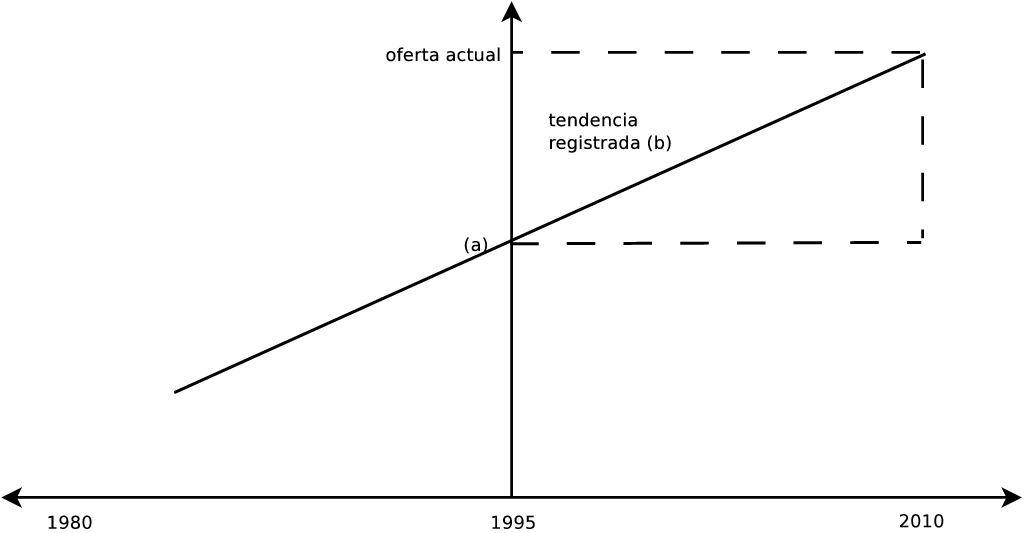
\includegraphics[scale=0.35]{img/oferta}
%\end{center}
%
%Se puede observar que mediante un calculo geométrico que:
%
%\begin{center}
%$\frac{oferta\_actual - a}{2010-1995} = b$
%\end{center}
%
%Donde b fue encontrado mediante investigación (punto anterior), por lo que es un dato conocido. Dando como resultado final para el intercepto:
%
%\begin{center}
%$a = oferta\_actual - 15b$
%\end{center}
%
%Reemplazando los valores actuales y la tendencia encontrada por investigación:
%
%\begin{center}
%a = 7 - 15b = \red{COLOCAR}\\
%b = \red{INVESTIGAR y COLOCAR, calcular lo de arriba}
%\end{center}
%
%Dando finalmente que:
%
%\begin{center}
%$oferta = a + bx$ \red{PONER CON VALORES REALES}
%\end{center}
%
